%欢迎来到:Someday's XeLaTeX Template For 冯如杯学术科技作品比赛
%开发者:Someday(BUAA-SCSE)
%维护: lawye(1874), nikkukun(1874)

\documentclass[zihao=-4]{ctexart}
%********************导言区宏包引入********************
\usepackage{xeCJK}
\usepackage{amssymb}
\usepackage{amsmath}
\usepackage{listings} %代码
\usepackage{graphicx}
\usepackage{multicol} %回车换段
\usepackage{xcolor}
\usepackage{geometry} %页面设置
\usepackage{fontspec}
\usepackage{times}
\usepackage{fancyhdr} %页眉页脚
\pagestyle{fancy}
\usepackage{float} %表格位置
\usepackage{titlesec} %设置
\usepackage{ctex}
\usepackage{gbt7714} %控制参考文献格式为国标
%********************导言区宏包引入********************
%********************第三方字体引入********************
%\setCJKmainfont[Path=fonts/,BoldFont=simhei.ttf,ItalicFont=simkai.ttf,SlantedFont=simfang.ttf]{simsun.ttc}
%中文字体涵盖黑体、宋体、楷体、仿宋
\setmainfont[Path=fonts/]{Times New Roman.ttf}
\setmonofont[Path=fonts/]{Courier New.ttf}
\setCJKfamilyfont{hwzs}[Path=fonts/]{STKzhongsong.ttf}%使用STZhogsong华文中宋字体
\newcommand{\zhongsong}{\CJKfamily{hwzs}}

%********************第三方字体引入********************


%********************中文字号设置********************
%\newcommand{\chuhao}{\fontsize{42pt}{\baselineskip}\selectfont}
\newcommand{\chuhao}{\fontsize{42pt}{0}}
\newcommand{\xiaochu}{\fontsize{36pt}{0}}
\newcommand{\yihao}{\fontsize{28pt}{0}}
\newcommand{\erhao}{\fontsize{21pt}{0}}
\newcommand{\xiaoer}{\fontsize{18pt}{0}}
\newcommand{\sanhao}{\fontsize{15.75pt}{0}}
\newcommand{\sihao}{\fontsize{14pt}{0}}
\newcommand{\xiaosi}{\fontsize{12pt}{0}}
\newcommand{\wuhao}{\fontsize{10.5pt}{0}}
\newcommand{\xiaowu}{\fontsize{9pt}{0}}
\newcommand{\liuhao}{\fontsize{7.875pt}{0}}
\newcommand{\qihao}{\fontsize{5.25pt}{0}}
%********************中文字号设置********************


%********************页边距设置********************
\geometry{left=3cm,right=2.5cm,top=2.5cm,bottom=2.5cm}
%页边距
%********************页边距设置********************
%********************

%欢迎来到:Someday's XeLaTeX Template
%开发者:Someday(BUAA-SCSE)
%任何问题或建议:欢迎关注微信公众平台“SomedayWill”,并在后台提问~

\begin{document}

%********************页眉页脚设置********************
\lhead{}%设置左页眉为空
\rhead{}%设置左页眉为空
%********************页眉页脚设置********************


%********************标题格式设置********************
\titleformat{\section}[block]{\LARGE\bfseries\centering}{\chinese{section}、}{1em}{}[]
\titleformat{\subsection}[block]{\Large\itshape\mdseries}{(\chinese{subsection})}{1em}{}[]
\titleformat{\subsubsection}[block]{\normalsize\bfseries}{\arabic{subsubsection}、}{.5em}{}[]
\titlespacing{\section}{0pt}{7.375pt}{7.375pt}
\titlespacing{\subsection}{0pt}{7pt}{7pt}
\titlespacing{\subsubsection}{0pt}{6pt}{6pt}
%\setcounter{secnumdepth}{0}%该命令取消了章标题前数字label
%\CTEXsetup[name={,、},number={\chinese{section}}]{section}
%\CTEXsetup[name={(,)},number={\chinese{subsection}}]{subsection}
%\CTEXsetup[name={,、},number={\arabic{subsubsection}}]{subsubsection}

%\titleformat{\section}[block]{\LARGE\bfseries}{\chinese{section}、}{1em}{}[]
%\titleformat{\subsection}[block]{\Large\itshape\mdseries}{(\chinese{subsection})}{1em}{}[]
%\titleformat{\subsubsection}[block]{\normalsize\arabic{subsubsection}、}{1em}{}[]

%\titleformat{\paragraph}[block]{\small\bfseries}{\arabic{paragraph}、}{1em}{}[]
%********************标题格式设置********************

%\setcounter{section}{-3}  %标题计数器
%\stepcounter{section}

%*******************行间距段前段后*******************
\linespread{1.8} %行间距为实际行间距乘以1.2,如此处实际为1.5倍行距
\setlength{\parskip}{0.5\baselineskip}
%*******************行间距段前段后*******************



%********************封面部分********************

\includegraphics[scale=1]{include_picture/xiaohui.png}
%格式控制部分
\par \  
\par \ 
\par \ 
\begin{center}

\includegraphics[scale=1]{include_picture/xiaoming.png}
\end{center}
%格式控制部分
\par \ 
\par \ 
\par \ 

\begin{center}
    \erhao\zhongsong{本模板由北航计算机学院Someday开发}
    \par \ 
    \erhao\zhongsong{本模板供所有用户免费使用,勿做商用}
\end{center}
%格式控制部分
\par \ 
\par \ 
\par \ 

\begin{center}
    \sihao
    \textbf{学院:计算机学院}
    \par \ 
    \textbf{本模板作者:Someday}
\end{center}

%格式控制部分
\par \ 
\par \  
\sanhao
\centerline{\textbf{二〇一七年七月}}

\pagenumbering{gobble} %封面无页码
%\thispagestyle{empty}


\renewcommand{\headrulewidth}{0pt}%没有页眉装饰线
\clearpage
\pagenumbering{roman} %摘要目录页小写罗马

\xiaosi
\section*{摘要}

欢迎来到:Someday's XeLaTeX Template

开发者:Someday(BUAA-SCSE)

\newpage
\section*{Abstract}

%********************摘要部分********************


%********************目录部分********************
\clearpage
\tableofcontents
\clearpage
%********************目录部分********************



\renewcommand{\headrulewidth}{0.4pt} %恢复页眉装饰线

%********************正文页眉部分********************
%\lhead{} 
\chead{本模板系北航计算机学院Someday所开发,供个人用户免费使用,勿做商用} %设置居中页眉
%********************正文页眉部分********************

\pagenumbering{arabic} %正文页码从1开始,用阿拉伯数字
\setcounter{page}{1} 


\section{公式和中文字体\ \ 和谐共处}

公式和中文字体和谐共处。

\subsection{LaTeX公式}

%********************正文部分********************
\begin{align*}
S=\iint\limits_{\Sigma}1 \ ds &= \int_0^{\pi}d\theta \int_0^{2\pi} r^2sin(\theta) d\phi \\
&= \int_0^{\pi}d\theta \int_0^{2\pi}\sin (\theta ) \left(\frac{1}{5} \sin (\theta  m) \sin (n \phi )+1\right)^2d\phi\\
&=\frac{4 \sin (\pi  m) \sin ^2(\pi  n)}{5 n-5 m^2 n}-\frac{\left(8 m^2+\cos (2 \pi  m)-1\right) \sin (4 \pi  n)}{200 \left(4 m^2-1\right) n}+\frac{\pi  \left(8 m^2+\cos (2 \pi  m)-1\right)}{50 \left(4 m^2-1\right)}+4 \pi\\
&=  \left(\frac{8 m^2}{50 \left(4 m^2-1\right)}+4\right)\pi
\end{align*}
%********************正文部分********************

\subsection{中文字体设置}

默认就是宋体。

调用加粗宋体:\textbf{黑体写在这里}

调用楷体:\textit{楷体写在这里}

调用仿宋:\textsl{仿宋写在这里}

调用黑体:\heiti{黑体写在这里}

\subsection{对齐方式}


%********************排版部分********************
\begin{center} 
居中文本第一行\\
居中文本第二行\\
\end{center}

\begin{flushright}
右对齐第一行\\
右对齐第二行\\
\end{flushright}

%********************排版部分********************


%欢迎来到:Someday's XeLaTeX Template
%开发者:Someday(BUAA-SCSE)

\section{图片与TeX子文件\ \ 信手拈来}

图片与TeX子文件信手拈来。

\subsection{图片}

%********************图片部分********************
\begin{figure}
    \centering
    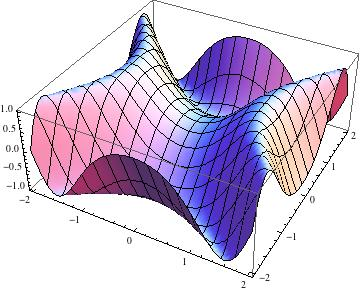
\includegraphics[scale=0.4]{include_picture/picture.jpg}
    \caption{插入图片}
\end{figure}
%********************图片部分********************

\subsection{引用Tex子文件}


%********************引用Tex子文件部分********************
*****以下内容均为引用部分*****\\
(1)解:$\because$ 根据和差化积 $\sin{\alpha}-\sin{\beta}=2\cos{\frac{\alpha+\beta}{2}}\sin{\frac{\alpha-\beta}{2}}$\\
$\therefore \sin{\sqrt{x+k}}-\sin{\sqrt{x}}=2\cos{\frac{\sqrt{x+k}+\sqrt{x}}{2}}\sin{\frac{\sqrt{x+k}-\sqrt{x}}{2}}$\\
$\therefore \lim\limits_{x \to +\infty}{\sin{\sqrt{x+k}}-\sin{\sqrt{x}}}
=\lim\limits_{x \to +\infty}{2\cos{\frac{\sqrt{x+k}+\sqrt{x}}{2}}\sin{\frac{\sqrt{x+k}-\sqrt{x}}{2}}}\\
=\lim\limits_{x \to +\infty}{cos{\frac{\sqrt{x+k}+\sqrt{x}}{2}}{\left(\sqrt{x+k}-\sqrt{x}\right)}}$\\
又$\lim\limits_{x \to +\infty}{\sqrt{x+k}-\sqrt{x}}=0,$
且$0\leqslant \left| \cos{\frac{\sqrt{x+k}+\sqrt{x}}{2}} \right|\leqslant 1$\\
$\therefore \lim\limits_{x \to +\infty}{\sin{\sqrt{x+k}}-\sin{\sqrt{x}}}
=\lim\limits_{x \to +\infty}{cos{\frac{\sqrt{x+k}+\sqrt{x}}{2}}{\left (\sqrt{x+k}-\sqrt{x}\right)}}=0$\\
(2)解:设
$$a_k=\begin{cases}
b_1-b_n &k=1,\\
b_k-b_{k-1} &2\leqslant k \leqslant n
\end{cases}$$\\
$\therefore$可以满足$\sum\limits_{k=1}^{n}{a_k}=0$,设定$b_0=b_n$\\
$\therefore \lim\limits_{x\to+\infty}{\sum\limits_{k=1}^{n}{{a_k}\sin{\sqrt{x+k}}}}
=\lim\limits_{x\to+\infty}{\sum\limits_{k=1}^{n}{{b_k-b_{k-1}}\sin{\sqrt{x+k}}}}\\
=\lim\limits_{x\to+\infty}{-\sum\limits_{k=1}^{n-1}{b_i{\left( \sin{\sqrt{x+k+1}}-\sin{\sqrt{x+k}} \right)}}-b_n{\left( \sin{\sqrt{x+1}}-\sin{\sqrt{x+k}} \right)}}$\\
又$\lim\limits_{x\to +\infty}{\sin{\sqrt{x+k}}-\sin{\sqrt{x}}}=0$\\
$\therefore \lim\limits_{x\to+\infty}{\sum\limits_{k=1}^{n}{\sin{\sqrt{x+k}}}}=0$\\
*****以上内容均为引用部分*****\\ %使用input不分页
%\include{includetex} %使用include将分页
%********************引用Tex子文件部分********************


%\titleformat*{\subsubsection}{\scshape\MakeLowercase}


\clearpage
\section{表格\ \ 提升逼格}

搞科研怎么能没有表格?\\

\subsection{表格}

%********************表格部分********************
关于表格的各种样式,请使用百度大法。\\
\begin{table}[H]
\caption{设置表格总长} 
\begin{tabular*}{12cm}{lll}
\hline  
Start & End  & Character Block Name \\  
\hline  
3400  & 4DB5 & CJK Unified Ideographs Extension A \\  
4E00  & 9FFF & CJK Unified Ideographs \\  
\hline  
\end{tabular*} 
\end{table} 
%********************表格部分********************


%********************代码部分********************

\section{代码片\ \ 程序员的最爱}
代码片永远是程序员的最爱,支持语法高亮,用法不妨百度。\\
\lstset{language=C}
\begin{lstlisting}
#include<iostream>
using namespace std;
int main()
{
    return 0;
}
\end{lstlisting}

%********************代码部分********************

\clearpage

\section{未完待续}

目前该模板基本可以应付日常论文写作需要,\par
尤其是对于我航学子,你们看看这个模板,是不是似曾相识,(尤其是能不能过冯如杯格式审查)。\par
限于精力,更多高级功能,请待作者再择良辰,Someday有朝一日还会回来。

\section{模板更新记录}

经123学长指正,Someday于2017.09.08进行一次重要更新,内容包括:\par
1、对中文字号的设置命令进行了修改,使用方法不变。\par
2、对仿宋字体所在的fontstyle进行了修改,以适应fontspec宏包。\par
3、将取消首页页码的命令改为:pagenumbering\{gobble\} \par

以上修正解决了以前版本中编译报错问题,当前版本在TeXLive2016环境下已经可以一次编译成功。 \par

编译命令如下: \par
cd\ <模板根目录> \par
xelatex main.tex \par

\par \ 
\par \ 

\section{模板新的更新记录}

lawye和nikkukun于2019.4.11开始维护该模板.

本次更新基于\it{第二十九届“冯如杯”学生学术科技作品竞赛论文撰写格式规范}\cite{格式}

\subsection{2019.4.11日更新记录}
\begin{enumerate}
    \item 修改参考文献格式

\end{enumerate}

% Reference
\newpage
\addcontentsline{toc}{section}{参考文献}%在目录中添加

\bibliography{library}
%\bibliographystyle{unsrt}



%欢迎来到:Someday's XeLaTeX Template
%开发者:Someday(BUAA-SCSE)



\end{document}


%欢迎来到:Someday's XeLaTeX Template
%开发者:Someday(BUAA-SCSE)
